\scanpage{68}
% block: nondegeneracy
un $\underline{\operatorname{Hom}}$ interne. On dit qu'un $F$-cristal $M$ est \uline{non dégénéré} s'il existe un entier $i\handwritten{\geqslant}0$ et un homomorphisme $V:M\handwritten{\longrightarrow}M^{\handwritten{\unsure{\sigma|\sigma'}}}$ tel que $VF=p^i$. Soit $\operatorname{FCriso}^{\inserted{\handwritten{+}}}\handwritten{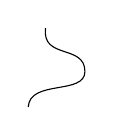
\begin{tikzpicture}[x=1cm,y=1cm,baseline=-.05cm]\draw[thin] (-.4,.6).. controls (-.45,.2) and (.1,.4)..(.1,.05).. controls (.1,-.25) and (-.6,-.05)..(-.62,-.4);\end{tikzpicture}}(k)$ la catégorie \deleted{des isocristaux} déduite de la catégorie des \deleted{\unsure{cr|er}} $F$-cri\deleted{z}staux non dégénérés en localisant par rapport à $p$ ; c'est donc une sous-$\otimes$-catégorie de celle des $F$-cristaux à isogénie près. On l'appellera la catégorie des $F$-\uline{isocristaux effectifs}, et on laissera tomber le qualificatif ``iso'' s'il n'y a pas de risque de confusion.

% block: Tate crystal and inversion
\uline{Le} $F$-\uline{isocristal de Tate\handwritten{\begin{tikzpicture}[x=1cm,y=1cm,baseline=-.05cm]\draw[thin] (-.1,-.4)--(.14,.45);\end{tikzpicture}}inverse}\inserted{$K(-1)$}\handwritten{\begin{tikzpicture}[x=1cm,y=1cm,baseline=-.1cm]\draw[thin] (0,.15).. controls (.05,-.1) and (-.2,-.1)..(-.7,-.1).. controls (-1,-.1) and (-1.3,-.2)..(-1.3,-.5);\end{tikzpicture}} est déduit du $F$\handwritten{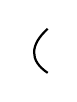
\begin{tikzpicture}[x=1cm,y=1cm,baseline=-.05cm]\draw[thick] (.12,.3).. controls (-.1,.1) and (-.12,-.1)..(.12,-.26);\end{tikzpicture}}-cristal\inserted{$W(-1)$}\handwritten{\begin{tikzpicture}[x=1cm,y=1cm,baseline=-.1cm]\draw[thin] (0,.15).. controls (.05,-.1) and (-.2,-.1)..(-.7,-.1).. controls (-1,-.1) and (-1.3,-.2)..(-1.3,-.5);\end{tikzpicture}} défini par le c\unsure{\deleted{i}r|\deleted{r}i}\unsure{\deleted{r}i|\deleted{i}r}stal \uline{unité}, avec $F_{K(-1)}=p.\operatorname{id}$ (cet $F$-cristal est évidemment non dégénéré !). On voit alors que $K(-1)$ est faiblement inversible, et on constate que lorsqu'on ajoute formellement à $\mathrm{FC}\overset{\handwritten{\mathord{\begin{tikzpicture}[x=1cm,y=1cm,baseline=0cm]\draw[thick] (0,0)--(.15,.015);\draw[thick] (.23,.025)--(.31,.005);\end{tikzpicture}}}}{\underset{r}{r}}\mathrm{iso}^{+}(k)$ \deleted{des} un in\handwritten{v}erse $K(1)$ de $K\handwritten{(-1),}$ alors on trouve une catégorie tannakienne sur $\underline{Q}_p$, ayant un foncteur fibre évident sur $K$; cette catégorie est notée $\operatorname{FCriso}(\unsure{\deleted{h}k|\deleted{k}h})$, et appelée \uline{catégorie des} $F$-\uline{\unsure{\deleted{c}i|\deleted{i}c}\unsure{\deleted{r}s|\deleted{s}r}ocristaux} \handwritten{(}ou simplement, s'il n'y \deleted{pa} a pas risque de confusion, des $F$-cristaux) sur $k$. $K(1)$ est le $F$\handwritten{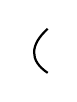
\begin{tikzpicture}[x=1cm,y=1cm,baseline=-.05cm]\draw[thick] (.12,.3).. controls (-.1,.1) and (-.12,-.1)..(.12,-.26);\end{tikzpicture}}-cristal de Tate, et on désigne par $M\handwritten{\mapsto}M(n)$ le foncteur de tensorisation par sa puissance tensorielle $n$.ème. Si $n=-m$, $m\handwritten{\geqslant}0$, ce fonc\deleted{te\unsure{u}}teur est induit par le foncteur sur les $F$-cristaux effectifs (sans iso\unsure{)} consistant à multiplier $F$ par $p^m$.

% block: crystals item 3
\handwritten{3.} Lorsque $k$ est parfait, désignant par $\handwritten{\sigma}$ l'automorphisme de Frobenius de $W=W(k)$, la donnée d'un $F$-cristal revient à la donnée d'un module de type fini $M$ sur $W$ muni d'un homomorphisme
\[
F_M\handwritten{\unsure{\deleted{=}:|\deleted{:}=|\div}}\quad M^{\handwritten{\unsure{\deleted{\sigma}\sigma|\sigma}}}=M\otimes_W(W,\handwritten{\sigma})\handwritten{\longrightarrow}M\ ,
\]
et le $F$\handwritten{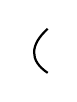
\begin{tikzpicture}[x=1cm,y=1cm,baseline=-.05cm]\draw[thick] (.12,.3).. controls (-.1,.1) and (-.12,-.1)..(.12,-.26);\end{tikzpicture}}-cristal est non dégénéré sss l'homomorphisme précédent est une isogénie \unsure{\deleted{n}i|\deleted{i}n|i}.e. est de rang égal à $\operatorname{rang}M$, ou encore sss il induit un isomorphisme après tensorisation par $K$. La catégorie \deleted{$\operatorname{Fiso}$} $\mathrm{Fc}\unsure{\deleted{\mathrm{ir}}\handwritten{ri}|\handwritten{ri}}\mathrm{s}(k)$ s'identifie alors à la catégorie des vectoriels de dimension finie
% archive sheet number: 67
